% !TeX root = ../../progress-sem1.tex
% 2.x โครงงาน งานวิจัยหรือผลิตภัณฑ์ที่เกี่ยวข้อง
\section{โครงงาน งานวิจัยหรือผลิตภัณฑ์ที่เกี่ยวข้อง}

\subsection{การประยุกต์ใช้ปัญญาประดิษฐ์ในการออกแบบ UX/UI}

\thaijustify{
  ในภาพรวม Tran-Truong et al.~\cite{trantruong2025genaiux} ทบทวนวรรณกรรมอย่างเป็นระบบจากงานวิจัย 68 ชิ้นที่ตีพิมพ์ระหว่างปี 2020 ถึง 2025 และจัดหมวดหมู่เครื่องมือ AI ตามขั้นของ Design Thinking ได้แก่ Empathize, Define, Ideate, Prototype และ Test ผลการทบทวนวรรณกรรมพบว่า AI ช่วยเร่งขั้น Prototype และ Test ได้มากที่สุดผ่านการทำงานอัตโนมัติ เช่น การสร้าง GUI การประเมินแบบ heuristic และการวิเคราะห์ข้อเสนอแนะเชิงคุณภาพด้วย LLM แต่งานวิจัยและเครื่องมือส่วนใหญ่ยังแยกกันตามแต่ละขั้น และยังขาดภาพรวมว่าเครื่องมือเหล่านี้ทำงานร่วมกันตลอดกระบวนการออกแบบอย่างไร อีกทั้งต้นแบบที่ AI สร้างมักดูดีในเบื้องต้นแต่ขาดความลึกเชิงฟังก์ชัน จึงยังต้องให้นักออกแบบคัดกรอง ข้อค้นพบนี้สอดคล้องกับแนวทางของโครงงานที่เชื่อมขั้น Prototype และ Test เข้าด้วยกันในแพลตฟอร์มเดียว
}

\thaijustify{
  งานวิจัยด้านการสร้าง UI ด้วย LLM แสดงให้เห็นทั้งศักยภาพและข้อจำกัดของเทคโนโลยี โดย Kolthoff et al. \cite{kolthoff2024} พบว่าการสร้าง UI ยังมีข้อผิดพลาดด้านการจัดวาง การตีความฟังก์ชัน และความไม่สอดคล้องขององค์ประกอบ เช่น สี ตัวอักษร และรูปแบบของ component ขณะที่ Ataei et al. \cite{ataei2025} ใช้ LLM Agents จำลองผู้ใช้เพื่อค้นหาความต้องการที่ไม่ได้ถูกระบุโดยตรง แต่ยังไม่ได้มุ่งเน้นการทดสอบต้นแบบกับผู้เข้าร่วมทดสอบแบบวนซ้ำ ส่วน Suh et al. \cite{suh2024} เสนอการใช้ LLM เพื่อสร้างและสำรวจทางเลือกหลายรูปแบบ แต่ยังไม่ได้เชื่อมทางเลือกเหล่านั้นเข้ากับการทดสอบการใช้งานและข้อเสนอแนะจากผู้เข้าร่วมทดสอบ
}

\thaijustify{
  อย่างไรก็ตาม LLM ยังมีอคติในการตัดสินใจ เช่น มีแนวโน้มตอบปฏิเสธมากเกินไปในงานที่ต้องตัดสินใจแบบใช่หรือไม่ใช่ โดยเฉพาะเมื่อโมเดลมีความรู้ไม่เพียงพอ ขณะที่การให้บริบทที่เกี่ยวข้องและการเปิดตัวเลือก ''ไม่ทราบ'' ช่วยลดอคตินี้ได้~\cite{song2025} ประเด็นนี้ต้องคำนึงถึงเมื่อให้ LLM จำแนกข้อเสนอแนะแบบเลือกตอบ เช่น การตัดสินว่าข้อเสนอแนะหนึ่งเป็นปัญหาการใช้งานหรือไม่ นอกจากนี้ การสร้าง Persona จากข้อมูลผู้ใช้ยังต้องอาศัยมนุษย์ช่วยระบุและตรวจสอบลักษณะที่สำคัญของแต่ละกลุ่ม~\cite{shin2024}
}

\thaijustify{
  จากข้อจำกัดดังกล่าว โครงงานนี้จึงนำ Generative AI มาใช้สนับสนุน
  กระบวนการแบบวนซ้ำตั้งแต่การสร้าง two-alternative UI การทดสอบกับผู้ใช้จริง การรวบรวมและวิเคราะห์ข้อเสนอแนะ ไปจนถึงการสังเคราะห์ข้อมูลสำหรับ Persona Artifact โดยให้นักออกแบบตรวจสอบและยืนยันผลการวิเคราะห์
  ก่อนเลือกข้อมูลที่จะนำไปใช้ปรับปรุงและสร้าง two-alternative UI สำหรับการทดสอบในรอบถัดไป
}

\subsection{แนวทางการปฏิสัมพันธ์ระหว่างมนุษย์กับปัญญาประดิษฐ์}
\thaijustify{
  Pourasad \& Maalej \cite{pourasad2025} ศึกษาการใช้ LLM เพื่อค้นหาปัญหาด้านการใช้งานของแอปพลิเคชัน และพบว่าปัญญาประดิษฐ์สามารถระบุปัญหาที่ถูกต้องได้บางส่วนแต่ยังพลาดปัญหาส่วนใหญ่ที่พบจากการทดสอบกับผู้ใช้ เนื่องจากปัญญาประดิษฐ์ วิเคราะห์จากข้อมูลของระบบและหน้าจอ แต่ไม่สามารถสะท้อนพฤติกรรม ความเข้าใจและปัญหาที่เกิดขึ้นระหว่างการใช้งานจริงของผู้ใช้ได้ทั้งหมด ดังนั้น ปัญญาประดิษฐ์จึงเหมาะกับการใช้เป็นเครื่องมือช่วยวิเคราะห์มากกว่าการทดแทนการทดสอบกับผู้ใช้จริง
}
\thaijustify{
  Tran-Truong et al.~\cite{trantruong2025genaiux} ชี้ในทำนองเดียวกันว่าบทบาทของนักออกแบบกำลังเปลี่ยนจากผู้ลงมือสร้างงานเอง (Maker) ไปเป็นผู้กำกับและคัดกรองผลลัพธ์ของ AI (Orchestrator และ Curator) และเกิดสิ่งที่ผู้วิจัยเรียกว่า Effort Paradox คือ AI ลดงานที่ต้องทำด้วยมือ แต่เพิ่มภาระทางความคิดในการเขียน prompt การตรวจสอบผลลัพธ์ และการกำกับด้านจริยธรรม ผู้วิจัยยังเตือนไม่ให้พึ่งพาผู้ใช้สังเคราะห์ (synthetic users) ที่ AI จำลองขึ้นโดยไม่ตรวจสอบ ข้อค้นพบนี้สนับสนุนให้โครงงานทดสอบกับผู้ใช้จริง และให้นักออกแบบตรวจและยืนยันผลของ AI ในแต่ละรอบ โดยแพลตฟอร์มช่วยลดภาระการตรวจสอบด้วยการแสดงขั้นตอนการทำงานของ AI และตรวจหน้าจออัตโนมัติก่อนส่งให้นักออกแบบ
}
\thaijustify{
  แนวคิดนี้สอดคล้องกับ Amershi et al. \cite{amershi2019} ที่เสนอให้ระบบปัญญาประดิษฐ์เปิดเผยความสามารถและข้อจำกัด รวมถึงเปิดโอกาสให้ผู้ใช้แก้ไขผลลัพธ์เมื่อปัญญาประดิษฐ์ทำงานผิดพลาด โครงงานนี้จึงให้ผู้ใช้จริงเป็นผู้ทดสอบและให้ข้อเสนอแนะ ส่วนปัญญาประดิษฐ์ทำหน้าที่ช่วยรวบรวม วิเคราะห์ และสรุปข้อมูล โดยให้นักออกแบบเป็นผู้ตรวจสอบและตัดสินใจขั้นสุดท้ายก่อนนำผลไปใช้ในรอบการออกแบบถัดไป
}

\subsection{ผลิตภัณฑ์และเครื่องมือในตลาดปัจจุบัน}
\thaijustify{
  จากการสำรวจผลิตภัณฑ์ที่เกี่ยวข้อง ณ ปัจจุบัน พบว่าเครื่องมือแต่ละกลุ่มมีจุดเด่นและข้อจำกัดที่ต่างกัน ได้แก่
  \begin{itemize}
    \item \textbf{เครื่องมือ A/B Testing (เช่น Kameleoon, Otter)} มักทำงานกับเว็บไซต์ที่พัฒนาเสร็จแล้ว (Live site) เพื่อวัดพฤติกรรมผู้ใช้ ซึ่งต่างจากโครงงานนี้ที่ทำงานกับต้นแบบก่อนการพัฒนา \cite{kameleoon, otterab}
      \begin{figure}[H]
        \centering
        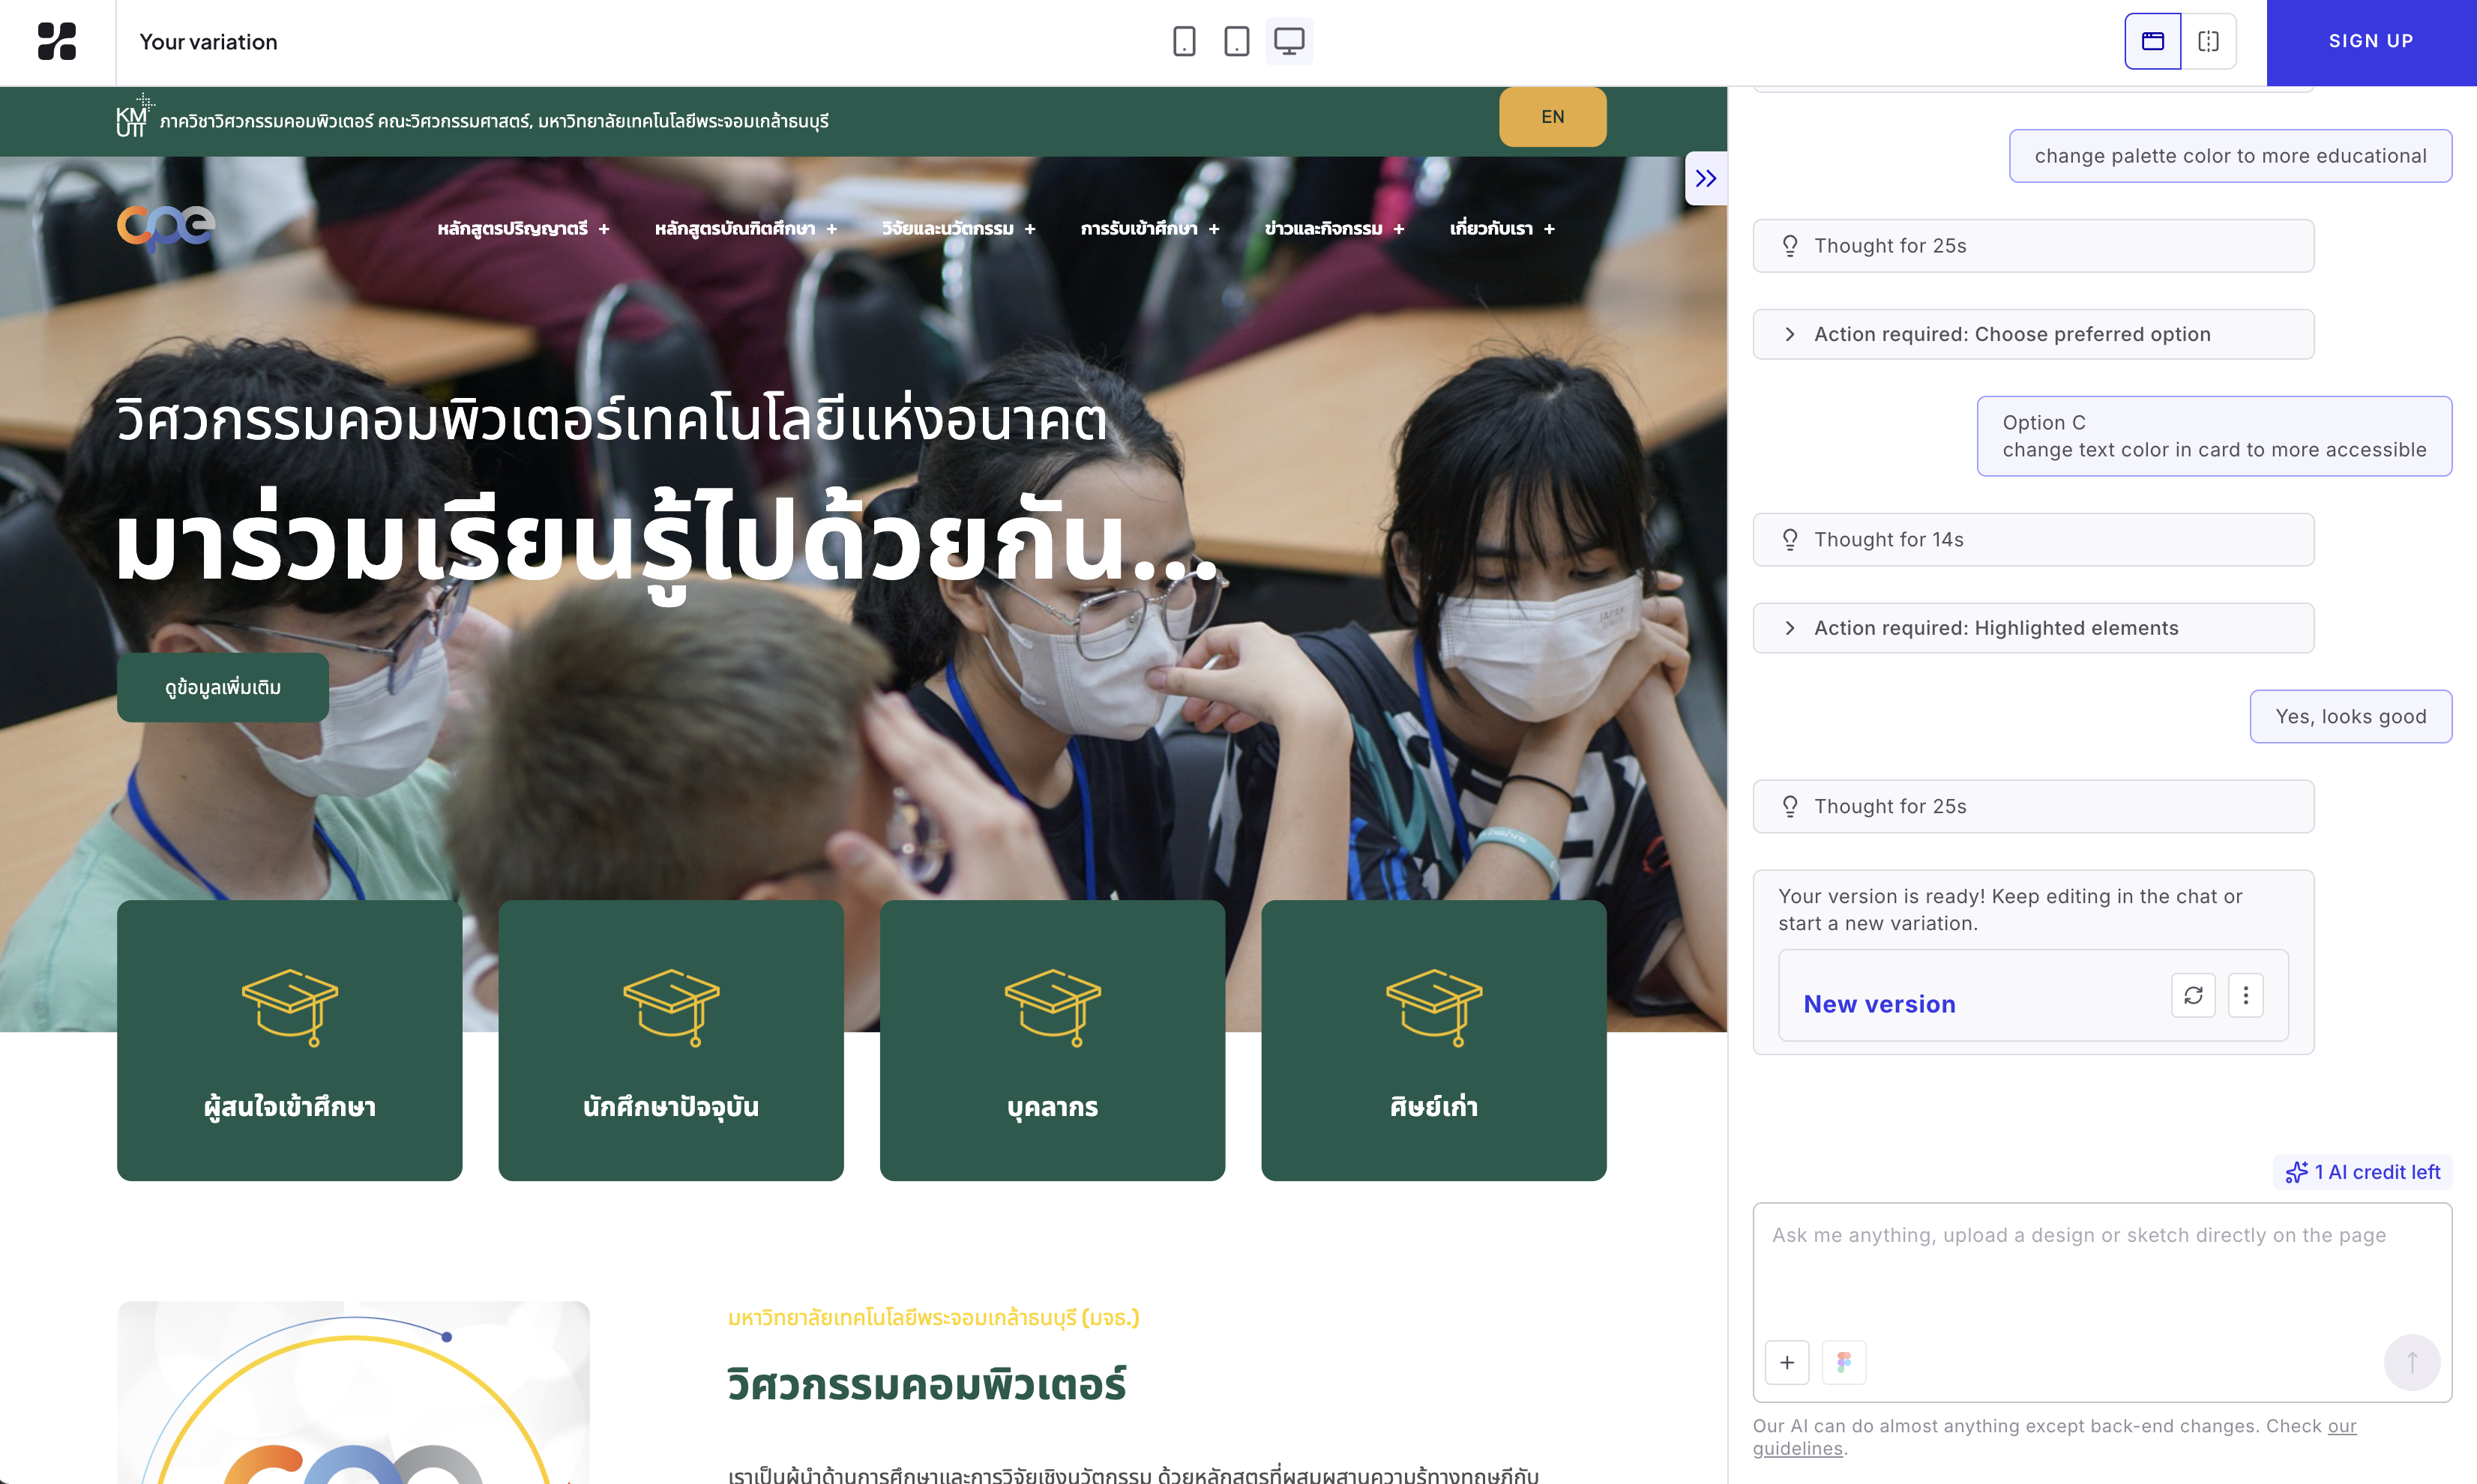
\includegraphics[
          width=0.5\textheight,
          height=0.95\linewidth,
          keepaspectratio,
          origin=c
        ]{figures/ch2-literature-review/kameleoon.png}
        \caption{แพลตฟอร์ม Kameleoon ใช้สำหรับการทำ A/B Testing}
        \label{fig:kameleoon}
      \end{figure}

    \item \textbf{เครื่องมือทดสอบผู้ใช้ก่อนเขียนโค้ด (เช่น Lyssna, Useberry)} มีฟังก์ชัน Preference testing สำหรับเปรียบเทียบดีไซน์หลายแบบ~\cite{lyssna,useberry} และ Lyssna เริ่มมี AI ช่วยสรุปธีมหลักจากคำตอบของผู้เข้าร่วมแล้ว~\cite{lyssna_synthesize} แต่จากการสำรวจเครื่องมือกลุ่มนี้ยังไม่ใช้ AI สร้างทางเลือกการออกแบบ (Variants) และยังไม่แยกปัญหาการใช้งาน (Pain point) ออกจากความชอบของผู้ใช้ในระบบเดียวกัน
      \begin{figure}[H]
        \centering
        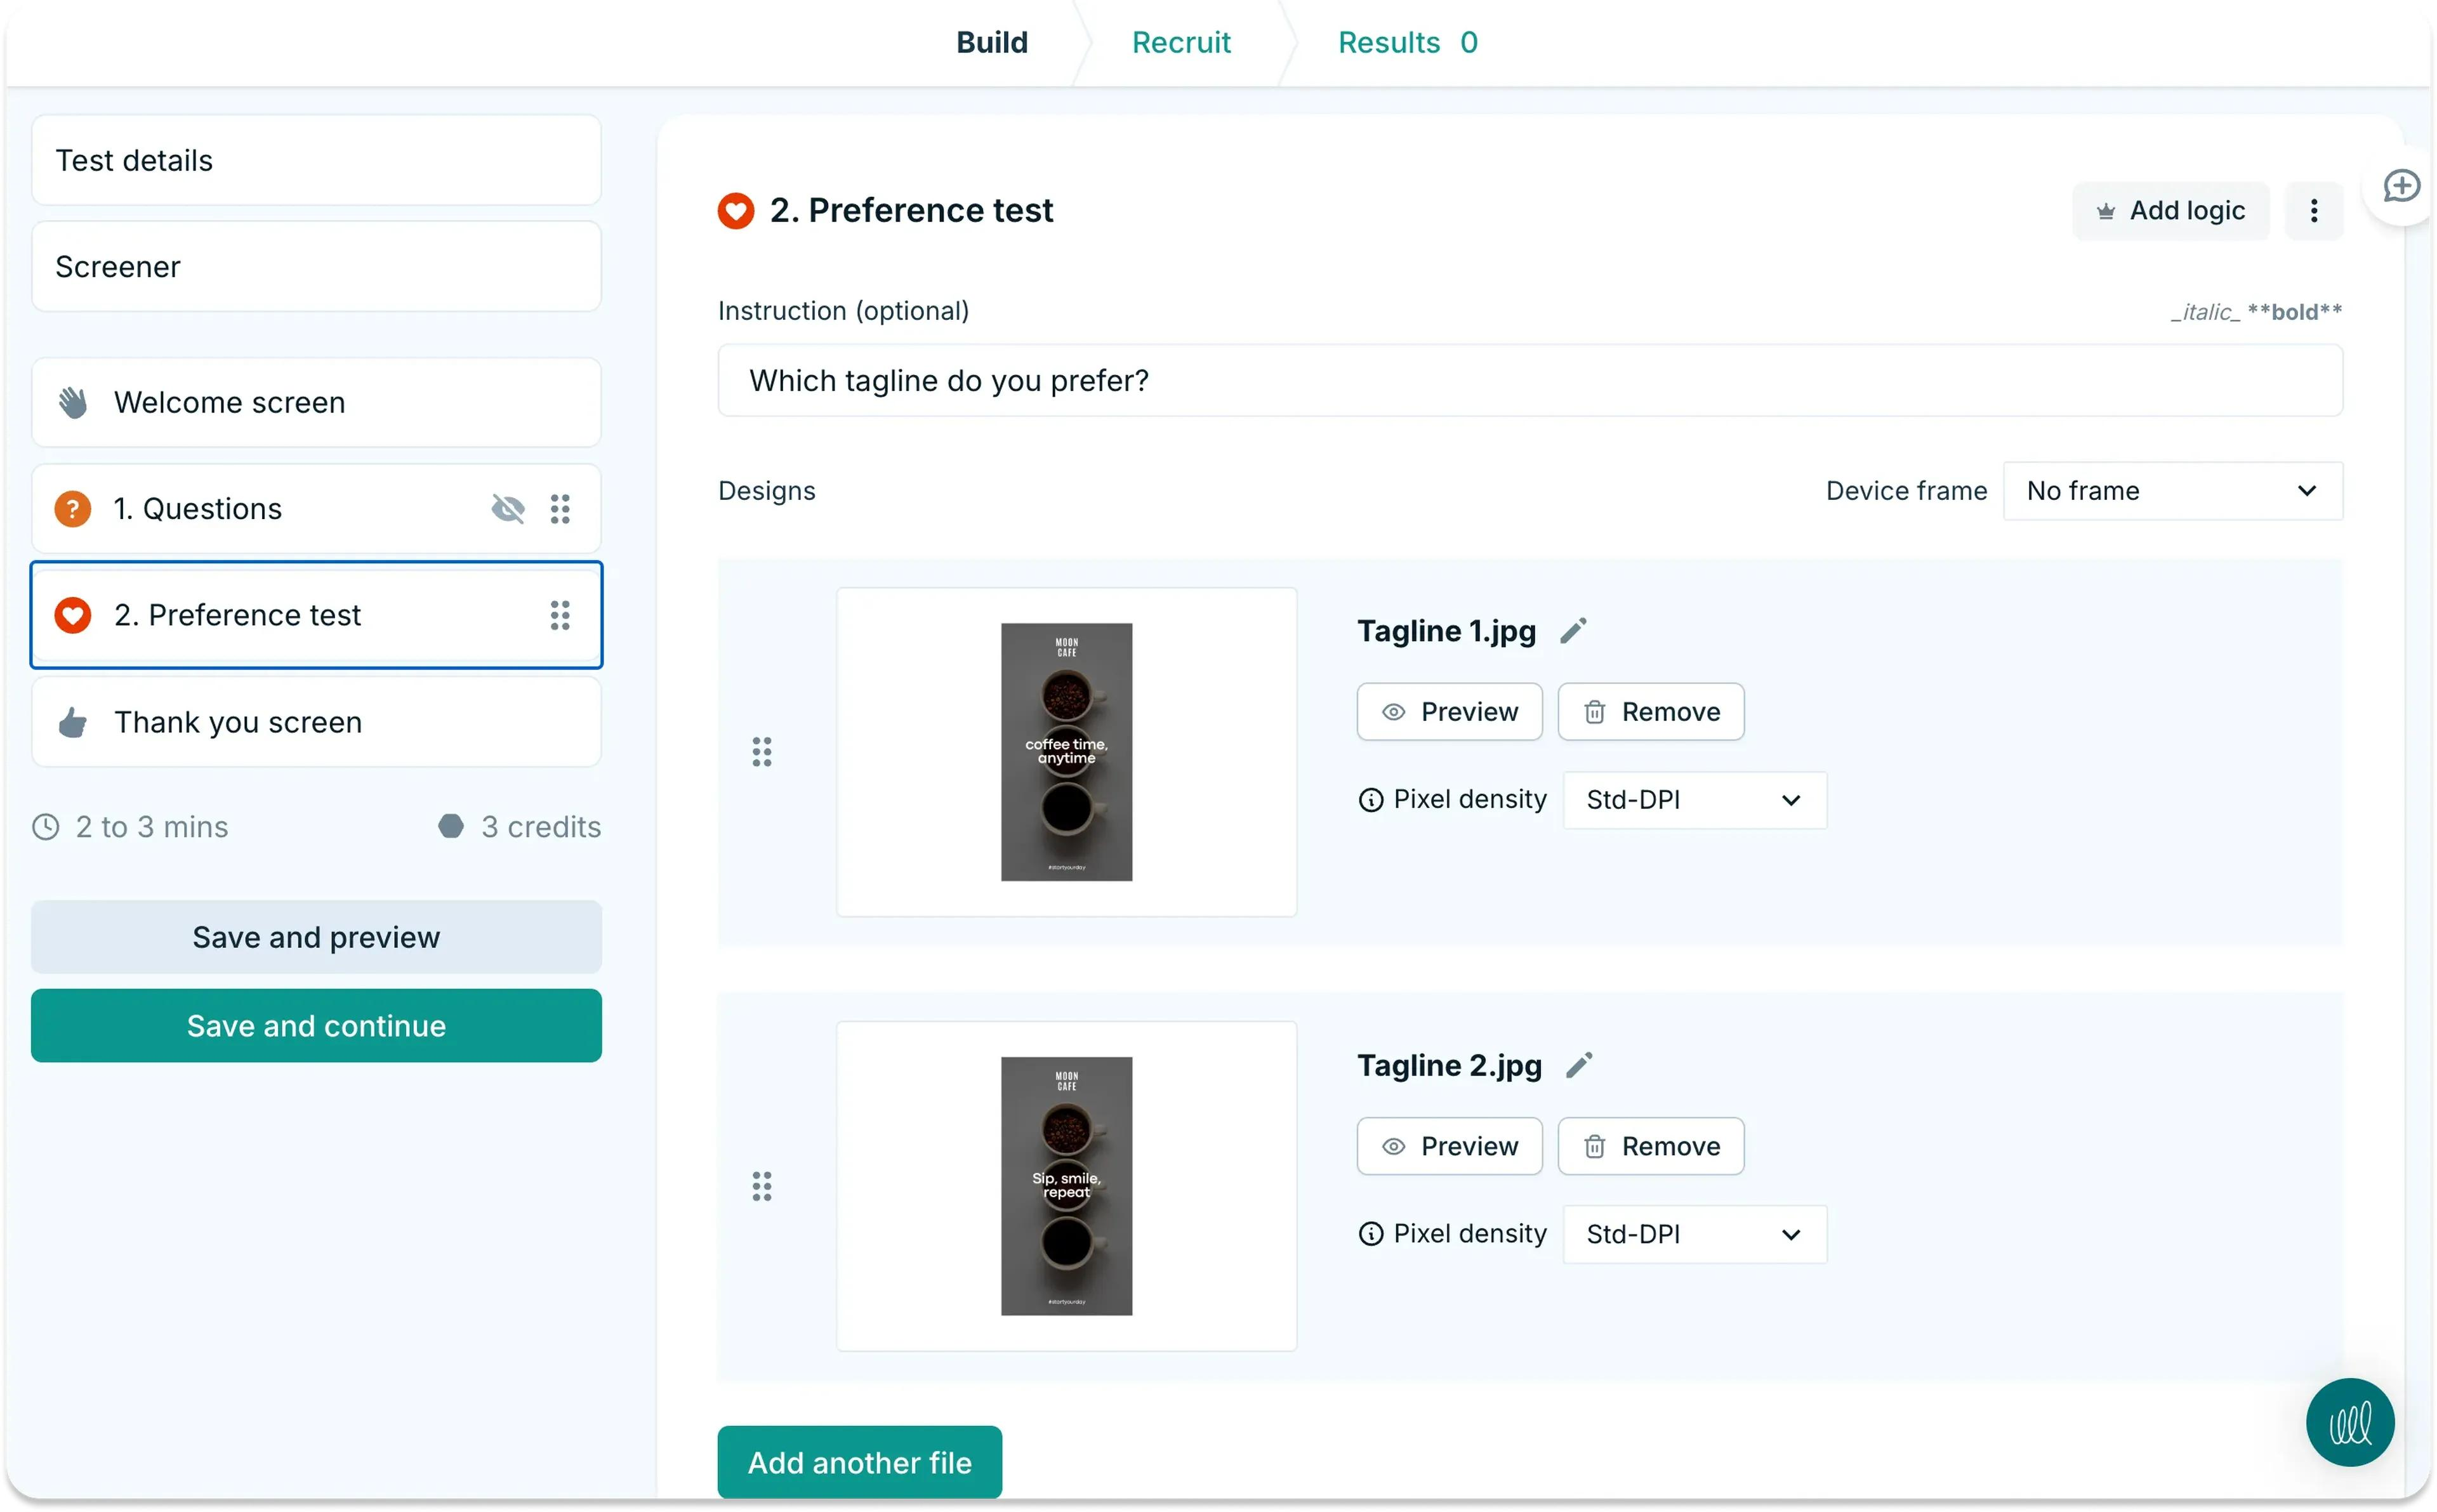
\includegraphics[
          width=0.5\textheight,
          height=0.95\linewidth,
          keepaspectratio,
          origin=c
        ]{figures/ch2-literature-review/lyssna.png}
        \caption{แพลตฟอร์ม Lyssna ใช้สำหรับการทดสอบการใช้งาน}
        \label{fig:lyssna}
      \end{figure}

    \item \textbf{เครื่องมือออกแบบที่มีปัญญาประดิษฐ์เป็นตัวช่วยในการทำงาน (เช่น Figma Make, Figma Agent)} สามารถสร้างต้นแบบหรือ Variants จากคำสั่งได้ โดย agent ของ Figma สร้าง Variants สำหรับ split test จาก component, token และ style ของ Design System~\cite{figma_agent} อย่างไรก็ตาม จากการสำรวจเครื่องมือกลุ่มนี้ยังไม่มีระบบรวบรวมข้อเสนอแนะจากผู้ทดสอบหลายกลุ่มเพื่อนำมาวิเคราะห์ร่วมกัน\cite{figma_agent}
      \begin{figure}[H]
        \centering
        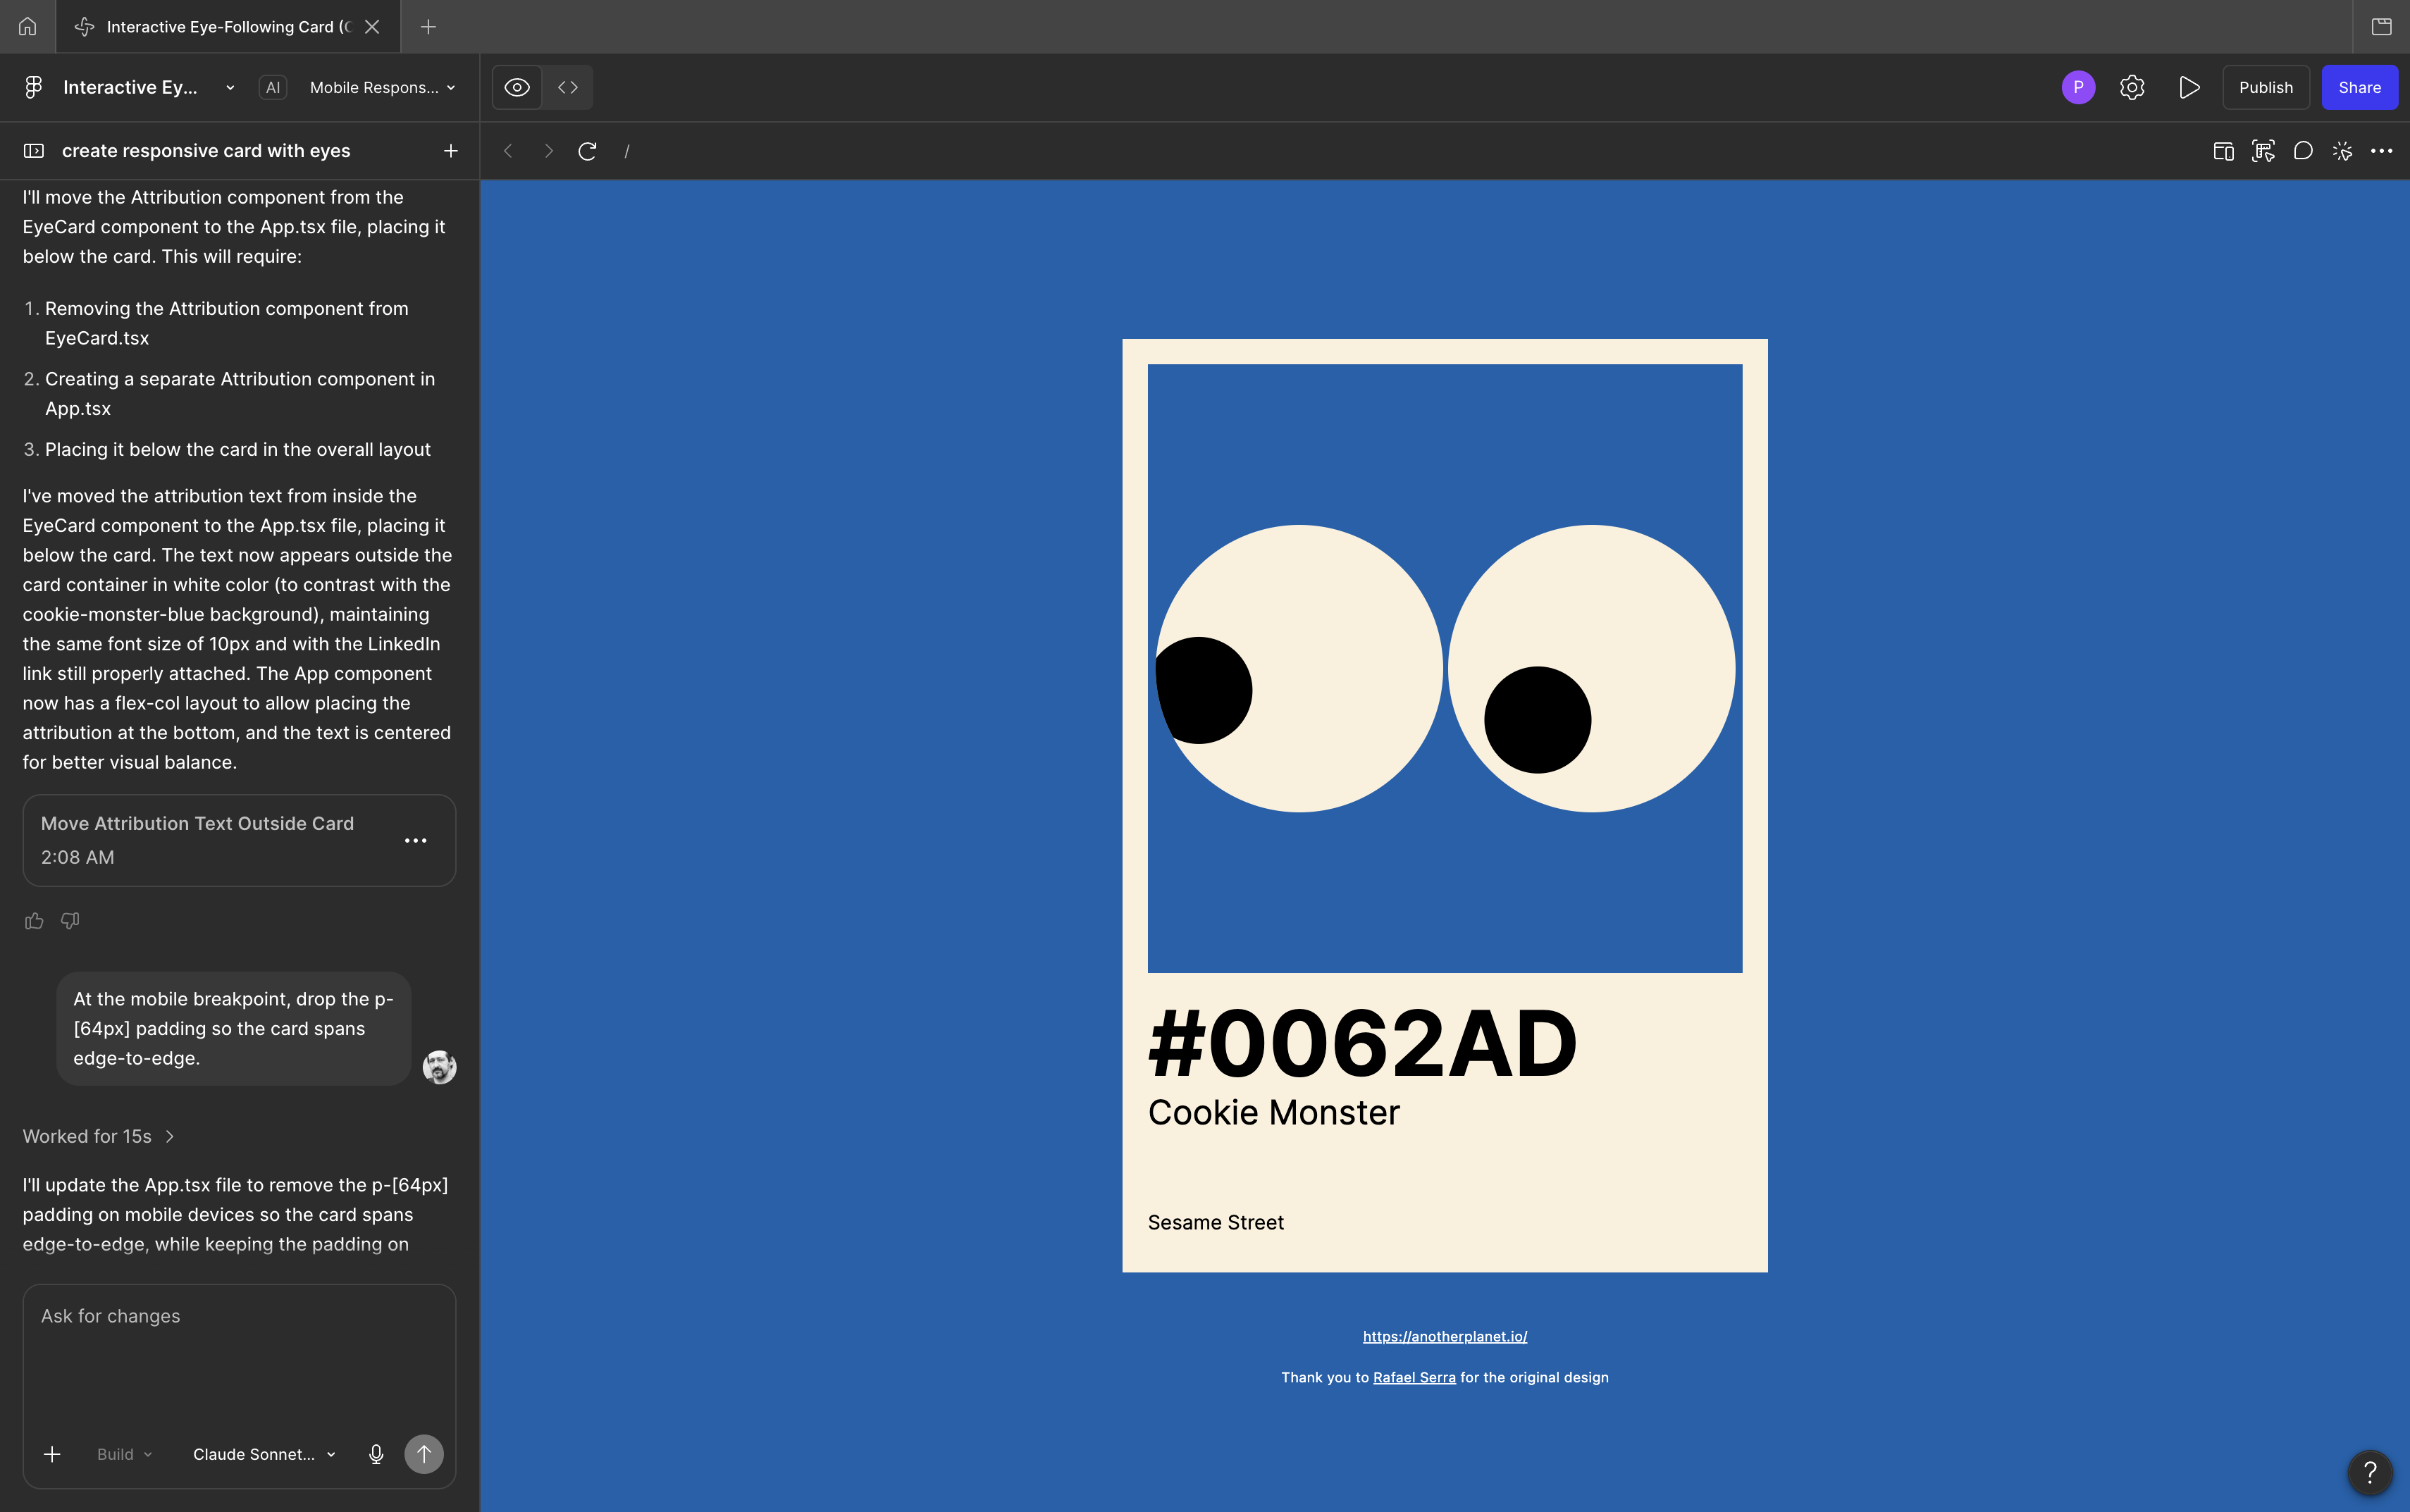
\includegraphics[
          width=0.5\textheight,
          height=0.95\linewidth,
          keepaspectratio,
          origin=c
        ]{figures/ch2-literature-review/figma-make.png}
        \caption{แพลตฟอร์ม Figma Make ใช้สำหรับสร้าง UI ด้วยภาษาธรรมชาติ}
        \label{fig:figma-make}
      \end{figure}

    \item \textbf{เครื่องมือตรวจงานด้วยหมุดคอมเมนต์ (เช่น BugHerd, Marker.io)} ให้ผู้ใช้ปักหมุดความคิดเห็นบนหน้าเว็บ พร้อมแนบภาพหน้าจอและข้อมูลทางเทคนิคโดยอัตโนมัติ~\cite{bugherd,markerio} และเริ่มนำ AI มาใช้จัดการข้อเสนอแนะแล้ว เช่น BugHerd เชื่อมต่อ AI agent ผ่าน MCP เพื่อช่วยคัดแยกงาน~\cite{bugherd_ai} แต่ยังขาดฟังก์ชันเปรียบเทียบสองทางเลือกและการจำแนกข้อเสนอแนะตามประเภทปัญหา
  \end{itemize}
}
